%        File: PlanVanAanpak_Inuits_LukasHanot.tex
%     Created: Fri Apr 12 06:00 PM 2019 C
% Last Change: Fri Apr 12 06:00 PM 2019 C
%
% Preamble
% ----
\title{Plan van aanpak}
\author{Lukas Hanot}
\date{\today{}}
\documentclass[a4paper]{article}
\setlength{\parskip}{1em}
\def\blankpage{%
  \clearpage%
  \thispagestyle{empty}%
  \addtocounter{page}{-1}%
  \null%
\clearpage}
% Packages
% ---
\usepackage{hyperref}
\usepackage{listings}
\usepackage{graphicx}
\usepackage{ulem}
\usepackage[utf8]{inputenc}
\usepackage[dutch]{babel}
\usepackage{pdfpages}

% Main document
% ---
\begin{document}
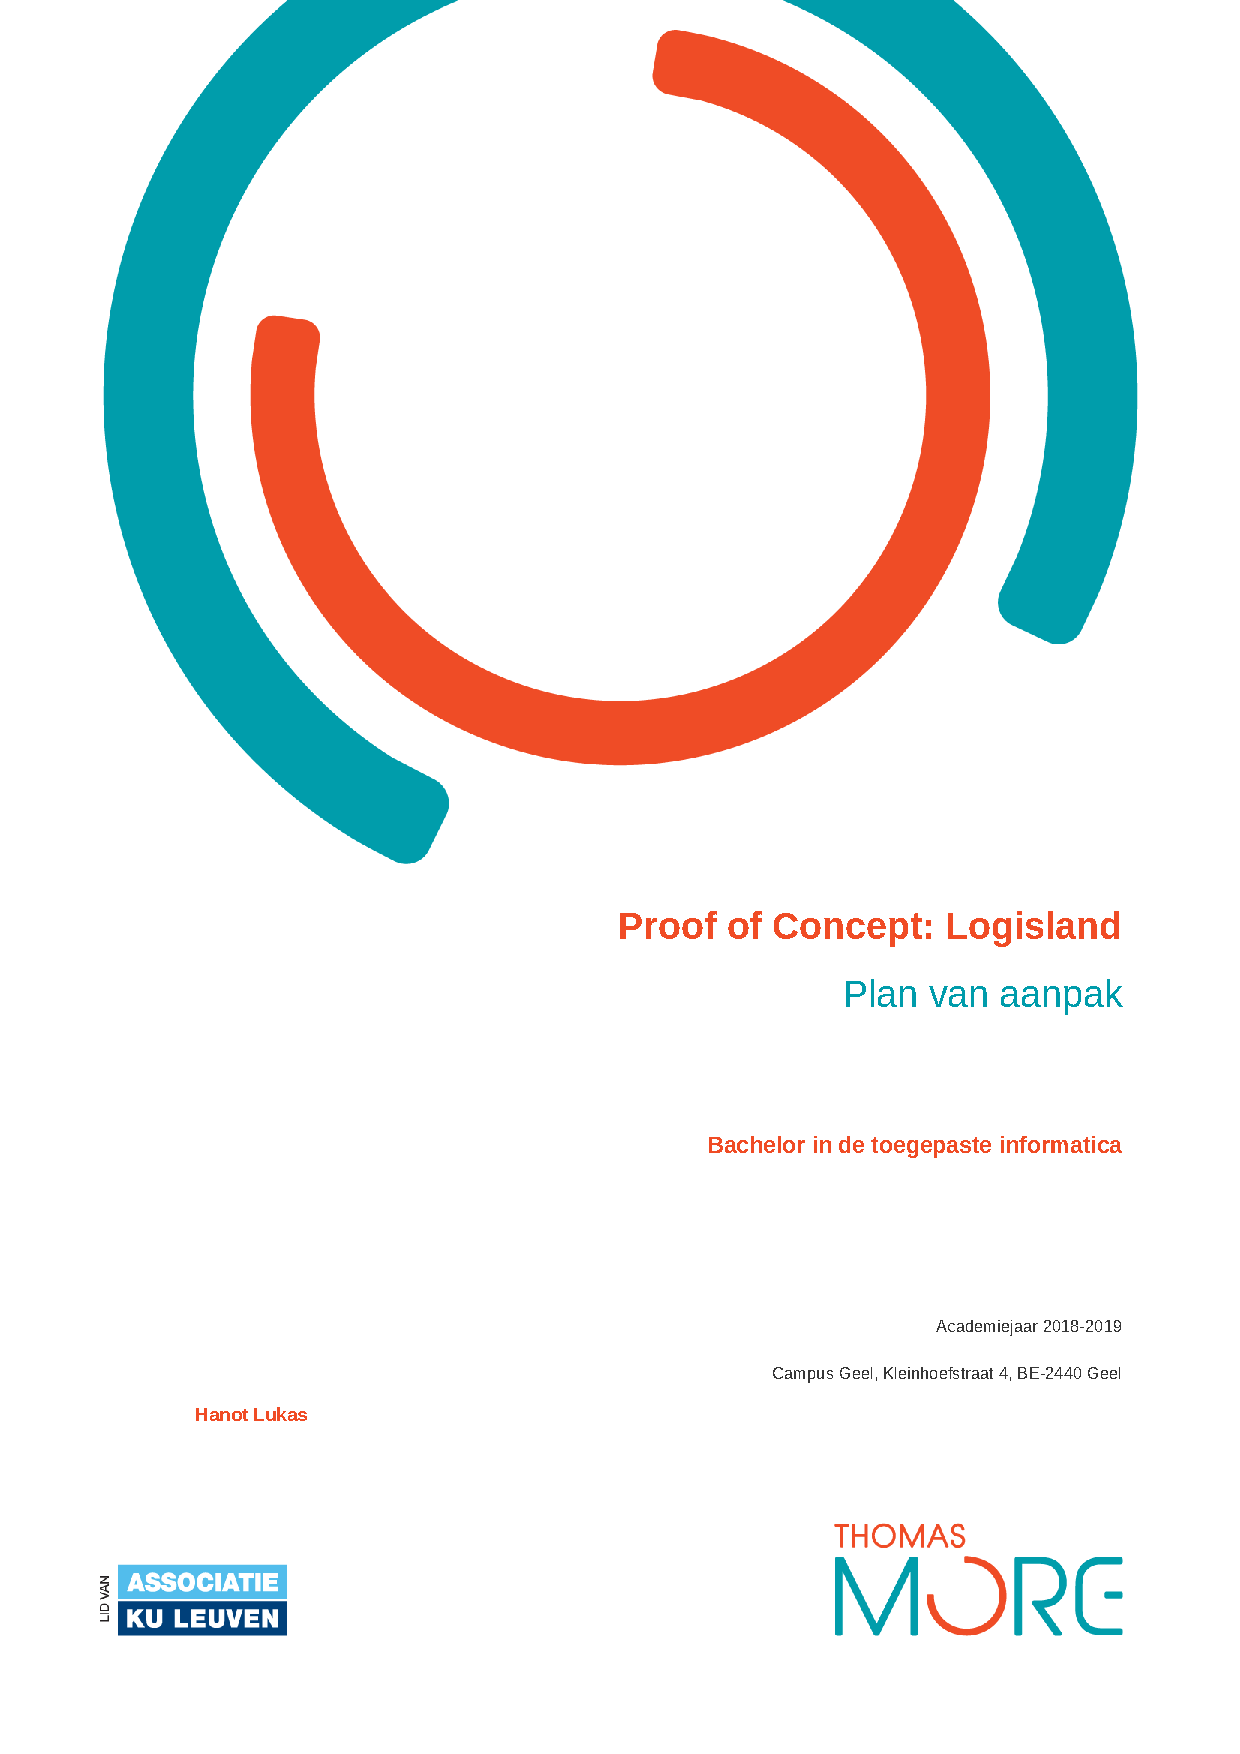
\includepdf[pages=-]{Voorblad.pdf}
\newpage
\blankpage
\pagenumbering{arabic}
\renewcommand{\contentsname}{}
\makeatletter
\renewcommand*\l@section{\@dottedtocline{1}{1.5em}{2.3em}}
\makeatother
\section*{Inhoudstafel}
\tableofcontents{}
\newpage{}

% Start of sections
% ---
\section*{Inleiding}
\addcontentsline{toc}{section}{\protect\numberline{}Inleiding}%
\begin{center}
``Every project is an opportunity to learn, to figure out problems and challenges, to invent and reinvent."
\end{center}
Deze woorden schreef \textit{David Rockwell} zeggen perfect wat deze stage voor mij betekent: een nieuw project en echte uitdaging om aan te gaan.
op 4 maart 2019 begint mijn stage bij Inuits, Open Source Innovators, gevestigt in Brasschaat zoekt dit bedrijf op maat gemaakte Open Source IT-oplossingen voor zijn klanten.
\par
Tijdens mijn stage bij Inuits moet ik als opdracht een Open Source applicatie bestuderen, testen en deployen om hierna te kunnen besluiten of deze al dan niet een aanwinst is voor het bedrijf.
\par
Voor dit onderzoek heb ik de hele periode van de stage de tijd al wordt er natuurlijk verwacht dat deze opdracht voltooid is voor het einde van de stage.
Mijn planning is daarom ook ruw ingeschat één maand testen/de werkomgeving leren kennen, één maand opzetten van de tool in de Inuits structuur en de laatste maand een werkende demo kunnen tonen aangevuld met een uitgebouwde conclusie voor de inzetbaarheid.


\newpage{}
\section{Stagebedrijf}
Inuits is opgericht in 2007 te Brasschaat en heeft al sinds 1997 ervaring met Open Source.
Binnen Inuits spreken we niet van afdelingen er zijn geen niveau's of muren om developers van systeembeheerders te scheiden.
Dit draagt natuurlijk bij aan het Open Source aspect van het bedrijf.
De werknemers zitten en werken samen om zo veel mogelijk informatie met elkaar te kunnen delen.
\par
Zonder deze muren focust het bedrijf zich wel op 3 technologische aspecten: \textbf{Dev}, \textbf{Ops}, en \textbf{DevOps}. Mijn stage focust zich voornamelijk op het Ops aspect waaronder onderdelen vallen zoals virtualisatie, monitoring en deployment. De eerste weken zal ik voornamelijk bezig zijn met een solo project waar ik binnen een eigen virtuele omgeving tools zal moeten opzetten. De samenwerking met developers zal hierdoor wel weinig aan bod komen dus hopelijk kan ik verder in de stage evolueren naar meer DevOps gerichte taken.

\newpage{}
\section{Aanleiding en achtergrond}
De tool waarmee ik deze stage aan de slag moet is Logisland, een applicatie die logs verzamelt en verwerkt.
Natuurlijk doet Inuits zelf al aan het verzamelen van logs met behulp van andere tools zoals Logstash en Icinga.
Dit levert een zeer robuust systeem op om problemen, die zich nu voor doen, op te lossen. maar minder om wederkerende problemen of tijd gebonden problemen te verwerken.
Hier komt Logisland binnenspringen: de tool slaagt erin om logs om te zetten in afzonderlijke tijdgebonden waarden die dan geanalyseerd kunnen worden.
\par
Inuits wil daarom dat ik een proof of concept en analyse uitvoer op zowel de bruikbaarheid, toepasbaarheid en werking van de Logisland applicatie. 

\newpage{}
\section{Doelstelling}
Mijn stageopdracht is het maken van een analyse van de Logisland applicatie, en voornamelijk gericht op bruikbaarheid ervan. 
Uit deze analyse verwacht Inuits te leren of de Logisland tool een aanwinst is in hun huidige infrastructuur en bij klanten.
Ik zal voor deze analyse dan ook een aantal duidelijke criteria moeten kunnen voorleggen alvorens ik een gegronde conclusie kan trekken.
\par
\begin{itemize}
\item Status van het Logisland project (toekomst, openheid, ondersteuning)
\item Staat van de documentatie 
\item Hardwarevereisten om de applicatie efficiënt te gebruiken
\item Algemene bruikbaarheid van de applicatie
\item Implementeerbaarheid met de huidige infrastructuur
\item Een werkende demo

\end{itemize}

\newpage{}
\section{Business case}
Wanneer mijn analyse voltooid is, zal het bedrijf hieruit zelf kunnen concluderen, afhankelijk van de gepresenteerde data, of de applicatie nuttig kan zijn. 
Nuttig zou in deze instantie betekennen dat de applicatie een groter inzicht zou geven op tijdgebonden problemen die zich voordoen binnen de huidige infrastructuur.
Deze problemen kunnen dan opgemerkt worden door analyse van de data die Logisland oplevert waardoor deze in de toekomst vermeden kunnen worden of waardoor de oorzaak, en niet enkel de symptomen, van een probleem wordt opgelost.
\par
De applicatie zou natuurlijk niet alleen een voordeel kunnen betekennen binnen de eigen infrastructuur maar zou ook bij klanten een meerwaarde kunnen geven. 
Momenteel biedt Inuits al bij klanten monitoring en metrics aan maar dit zou natuurlijk nog uitgebreid kunnen worden met tijdgebonden analyses waardoor problemen op voorhand al vermeden kunnen worden.
Dit soort analyses is wel enkel mogelijk met degelijke tools, waarop men kan vertrouwen dat de data die eruit komt correct en bruikbaar is.

\newpage{}
\section{Fasering}
De planning die ik mezelf opleg voor het project beslaat de hele stage.
Vanwegen de complexiteit die aangegeven is door mijn stagementor voor dit project gun ik mezelf een ruim en los schema zodat er tijd is om te leren en groeien.
Het doel is om dit project af te krijgen tijdens de gekregen tijd. Als dit eerder lukt zijn er nog andere projecten om uit te voeren maar we werken stap voor stap.
\par
\paragraph{Week 1 \& 2} Bekend worden met de werkwijze binnen Inuits.
\paragraph{Week 3 \& 4} De applicatie deployen in een lokale virtuele omgeving (Virtualbox).
\paragraph{Week 5 \& 6} De Logisland tool deployen in de Inuits infrastructuur.
\paragraph{Week 7 \& 8} Logs vanuit de echte infrastructuur verwerken in Logisland.
\paragraph{Week 9 \& 10} De records die uit Logisland komen analyseren en omvormen tot rapporten.
\paragraph{Week 11 \& 12} Demo opzetten waarmee een probleem kan worden opgespoord.
\paragraph{Week 13} Proof of concept en conclusie presenteren aan stagementor.

\newpage{}
\section{Informatie en rapportering}
Communicatie zal gevoerd worden enerzijds dankzij de tools die al binnen Inuits voor handen zijn en anderzijds de opgelegde communicatie kanalen die de school hanteert.
\par
Binnen Inuits zijn er 3 grote tools die dienen om mensen op de hoogte te houden.De grootste van de 3 is Rocketchat: deze instant messenger zorgt ervoor dat iedereen binnen het bedrijf direct aanspreekbaar is en gemakkelijk kan communiceren.
Dan volgt 2 maal de wekelijkse Standup meetings over meet.jit.si, een online video conferencing platform, waar iedereen een update geeft over waaraan hij/zij bezig is en mogelijk problemen ondervind.
En als laatste is er Redmine een project tracking tool waarop mensen updates kunnen plaatsen van de projecten waar ze aan werken of gaan aan werken.
\par
De school heeft een aantal vaste praktijken die zei toepassen om het verloop van de stages te volgen.
De meest voorkomende updates zijn de logboeken die de student bijhoud en doorstuurt naar zijn/haar begeleider.
Hierin wordt dagelijks bijgehouden waaraan de student bezig is en of hij/zij ergens mee vastzit. Ik ga dit waarschijnlijk maken in een online word document op onedrive omdat deze gemakkelijk te delen is met Mr. Portier.
\par
Dan is voor mij persoonlijk nog een terugkoppel moment, als Mr. Portier tijd heeft, mogelijk na de les Windows Server Advanced die ik elke dinsdag heb. 
Windows Server Advanced is een tweede jaars vak dat ik nog moet volbrengen dat samenvalt tijdens de stage waardoor ik elke dinsdag op school moet zijn.
\par
De terugkommomenten zijn natuurlijk ook een belangrijk onderdeel van de communicatie met de stagebegeleider. Hier wordt niet alleen uitleg gegeven over de bachelorproef maar wordt ook feedback over de documentatie en communicatie van de stagair.
\end{document}



